\documentclass[tikz,border=0pt]{standalone}
\usetikzlibrary{calc}
% Palette: the 3D gym's colours (crates/core/src/mesh.rs, data/shaders/scene.frag).
\definecolor{sky}{HTML}{DCE6EE}
\definecolor{skyhi}{HTML}{F2F6F9}
\definecolor{wall}{HTML}{EDE6D3}
\definecolor{walldark}{HTML}{D6CCB4}
\definecolor{stripeblue}{HTML}{2F5CBF}
\definecolor{stripegold}{HTML}{F8C537}
\definecolor{window}{HTML}{CFE6FF}
\definecolor{windowlit}{HTML}{F6FBFF}
\definecolor{wood}{HTML}{DBA86B}
\definecolor{wooddark}{HTML}{B98549}
\definecolor{woodline}{HTML}{C9965A}
\definecolor{mat}{HTML}{2961CC}
\definecolor{matlit}{HTML}{4A82E8}
\definecolor{matdark}{HTML}{1C4597}
\definecolor{matseam}{HTML}{16377A}
\definecolor{red}{HTML}{DD3D38}
\definecolor{redlit}{HTML}{F06A5E}
\definecolor{reddark}{HTML}{A92A27}
\definecolor{yellow}{HTML}{F9C02E}
\definecolor{yellowlit}{HTML}{FFDB6B}
\definecolor{yellowdark}{HTML}{C9961C}
\definecolor{green}{HTML}{3FA866}
\definecolor{greenlit}{HTML}{62C98A}
\definecolor{greendark}{HTML}{2C7D4B}
\definecolor{pink}{HTML}{F27A93}
\definecolor{pinklit}{HTML}{F7A1B3}
\definecolor{orange}{HTML}{F28A2E}
\definecolor{orangelit}{HTML}{F7AE66}
\definecolor{orangedark}{HTML}{C2671A}
\definecolor{sky2}{HTML}{7FB8F0}
\definecolor{purple}{HTML}{8B5CC8}
\definecolor{skin}{HTML}{F2C49A}
\definecolor{skinlit}{HTML}{F8D8B8}
\definecolor{skindark}{HTML}{D9A47A}
\definecolor{skinb}{HTML}{B9835A}
\definecolor{skinbdark}{HTML}{93653F}
\definecolor{shirt}{HTML}{E2463F}
\definecolor{shirtdark}{HTML}{B23430}
\definecolor{shirtb}{HTML}{2F7DD8}
\definecolor{shirtbdark}{HTML}{225DA6}
\definecolor{shorts}{HTML}{21305A}
\definecolor{shortsdark}{HTML}{151F3D}
\definecolor{shoe}{HTML}{FFFFFF}
\definecolor{shoedark}{HTML}{D8DDE3}
\definecolor{hair}{HTML}{4A2F1C}
\definecolor{band}{HTML}{F8C537}
\definecolor{chick}{HTML}{FBE48F}
\definecolor{chicklit}{HTML}{FFF2BE}
\definecolor{chickdark}{HTML}{DCC064}
\definecolor{comb}{HTML}{E2302E}
\definecolor{beak}{HTML}{F28A2E}
\definecolor{noodle}{HTML}{57D163}
\definecolor{noodledark}{HTML}{3A9E45}
\definecolor{ball}{HTML}{D8302B}
\definecolor{balldark}{HTML}{A5211D}
\definecolor{balllit}{HTML}{F0645D}
\definecolor{duck}{HTML}{FFD12E}
\definecolor{duckdark}{HTML}{E0A814}
\definecolor{foam}{HTML}{2F6BE0}
\definecolor{foamdark}{HTML}{214FAD}
\definecolor{white}{HTML}{FFFFFF}
\definecolor{sand}{HTML}{EDCB85}
\definecolor{sandlit}{HTML}{F7E2AE}
\definecolor{sanddark}{HTML}{C9A35E}
\definecolor{camel}{HTML}{D6A35F}
\definecolor{cameldark}{HTML}{A97A3F}
\definecolor{lizard}{HTML}{66C752}
\definecolor{lizarddark}{HTML}{3A8A34}
\definecolor{potclay}{HTML}{D06A3D}
\definecolor{glass}{HTML}{D6EAF2}
\definecolor{stick}{HTML}{7CF25C}
\definecolor{sticklit}{HTML}{C8FFB0}
\definecolor{night}{HTML}{24222B}
\definecolor{nightlit}{HTML}{3A3744}
\definecolor{gold}{HTML}{F5C231}
\definecolor{goldlit}{HTML}{FFE07A}
\definecolor{golddark}{HTML}{B98A12}
\definecolor{wrap}{HTML}{F0EBD6}
\definecolor{wrapdark}{HTML}{C9C2A8}
\definecolor{ink}{HTML}{1E2B45}
\definecolor{netline}{HTML}{9AA9BF}
\definecolor{glow}{HTML}{FFF4C2}
\definecolor{stone}{HTML}{8C8C93}
\definecolor{stonelit}{HTML}{A9A9B0}
\definecolor{crystal}{HTML}{8CF2D9}
\definecolor{crystaldark}{HTML}{4CBFB2}
\definecolor{brown}{HTML}{73492E}
\definecolor{brownlit}{HTML}{93623F}
\definecolor{paper}{HTML}{F4F4F0}
\definecolor{paperdark}{HTML}{CDD1D8}
\begin{document}
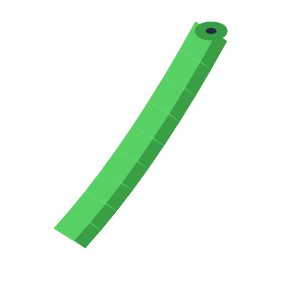
\begin{tikzpicture}[x=1cm,y=1cm]
\useasboundingbox (0,0) rectangle (3,3);
\fill[noodle] (0.33,0.45) -- (0.73,0.2) -- (0.93,0.428) -- (0.53,0.678) -- cycle;
\fill[noodledark] (0.6,0.3) -- (0.73,0.2) -- (0.93,0.428) -- (0.8,0.528) -- cycle;
\fill[noodle] (0.53,0.678) -- (0.93,0.428) -- (1.13,0.672) -- (0.73,0.922) -- cycle;
\fill[noodledark] (0.8,0.528) -- (0.93,0.428) -- (1.13,0.672) -- (1,0.772) -- cycle;
\fill[noodle] (0.73,0.922) -- (1.13,0.672) -- (1.33,0.932) -- (0.93,1.182) -- cycle;
\fill[noodledark] (1,0.772) -- (1.13,0.672) -- (1.33,0.932) -- (1.2,1.032) -- cycle;
\fill[noodle] (0.93,1.182) -- (1.33,0.932) -- (1.53,1.208) -- (1.13,1.458) -- cycle;
\fill[noodledark] (1.2,1.032) -- (1.33,0.932) -- (1.53,1.208) -- (1.4,1.308) -- cycle;
\fill[noodle] (1.13,1.458) -- (1.53,1.208) -- (1.73,1.5) -- (1.33,1.75) -- cycle;
\fill[noodledark] (1.4,1.308) -- (1.53,1.208) -- (1.73,1.5) -- (1.6,1.6) -- cycle;
\fill[noodle] (1.33,1.75) -- (1.73,1.5) -- (1.93,1.808) -- (1.53,2.058) -- cycle;
\fill[noodledark] (1.6,1.6) -- (1.73,1.5) -- (1.93,1.808) -- (1.8,1.908) -- cycle;
\fill[noodle] (1.53,2.058) -- (1.93,1.808) -- (2.13,2.132) -- (1.73,2.382) -- cycle;
\fill[noodledark] (1.8,1.908) -- (1.93,1.808) -- (2.13,2.132) -- (2,2.232) -- cycle;
\fill[noodle] (1.73,2.382) -- (2.13,2.132) -- (2.33,2.472) -- (1.93,2.722) -- cycle;
\fill[noodledark] (2,2.232) -- (2.13,2.132) -- (2.33,2.472) -- (2.2,2.572) -- cycle;
\fill[noodle] (1.93,2.722) -- (2.33,2.472) -- (2.53,2.828) -- (2.13,3.078) -- cycle;
\fill[noodledark] (2.2,2.572) -- (2.33,2.472) -- (2.53,2.828) -- (2.4,2.928) -- cycle;
\fill[noodledark] (2.33,2.958) ellipse (0.21 and 0.12);
\fill[ink] (2.33,2.958) ellipse (0.07 and 0.04);
\end{tikzpicture}
\end{document}
